\begin{figure}[htbp]
\centering
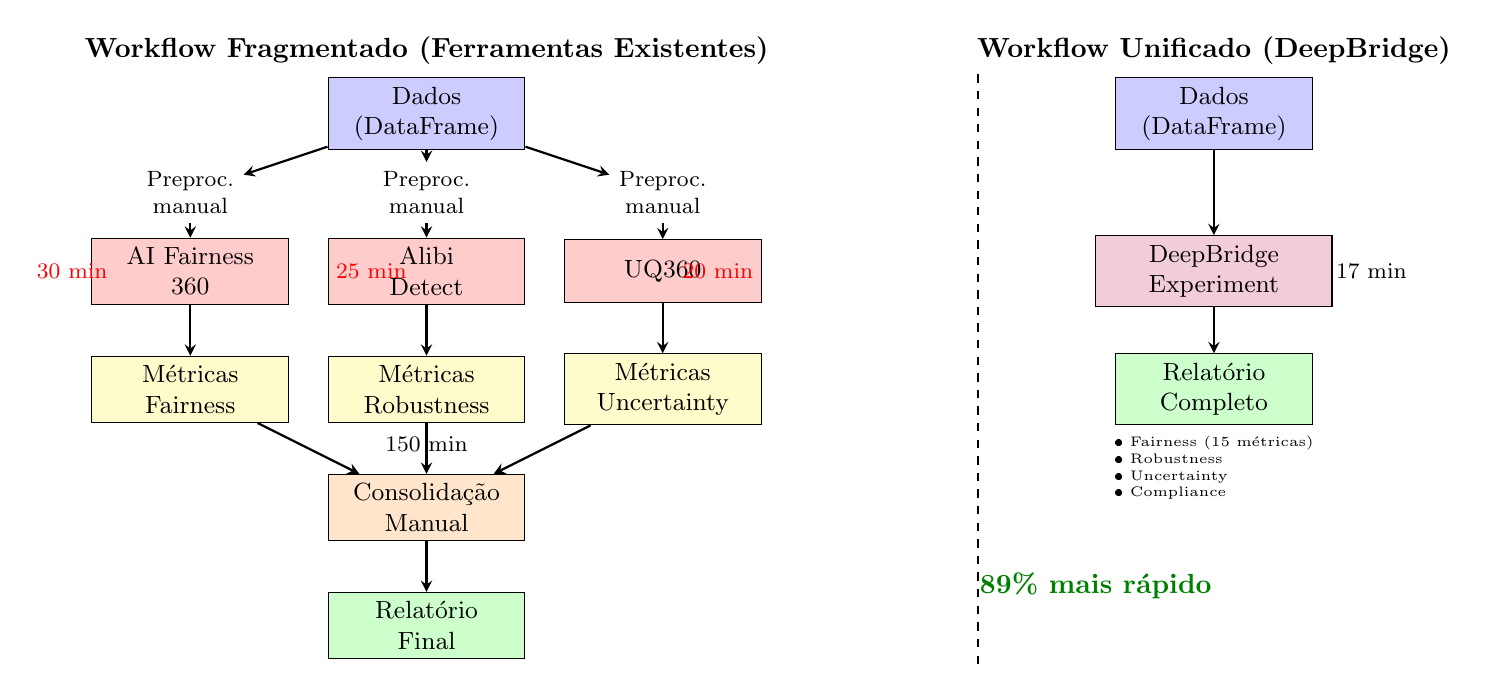
\begin{tikzpicture}[
    box/.style={rectangle, draw, minimum width=2.5cm, minimum height=0.8cm, align=center, font=\small},
    arrow/.style={->, >=stealth, thick},
    label/.style={font=\footnotesize, align=center}
]

% Workflow fragmentado
\node[box, fill=blue!20] (data) at (0,0) {Dados \\ (DataFrame)};

% Ferramentas fragmentadas
\node[box, fill=red!20] (aif360) at (-3,-2) {AI Fairness\\360};
\node[box, fill=red!20] (alibi) at (0,-2) {Alibi\\Detect};
\node[box, fill=red!20] (uq360) at (3,-2) {UQ360};

% Pré-processamento manual
\node[label] (preproc1) at (-3,-1) {Preproc.\\manual};
\node[label] (preproc2) at (0,-1) {Preproc.\\manual};
\node[label] (preproc3) at (3,-1) {Preproc.\\manual};

% Setas de pré-processamento
\draw[arrow] (data) -- (preproc1);
\draw[arrow] (data) -- (preproc2);
\draw[arrow] (data) -- (preproc3);
\draw[arrow] (preproc1) -- (aif360);
\draw[arrow] (preproc2) -- (alibi);
\draw[arrow] (preproc3) -- (uq360);

% Resultados
\node[box, fill=yellow!20] (res1) at (-3,-3.5) {Métricas\\Fairness};
\node[box, fill=yellow!20] (res2) at (0,-3.5) {Métricas\\Robustness};
\node[box, fill=yellow!20] (res3) at (3,-3.5) {Métricas\\Uncertainty};

\draw[arrow] (aif360) -- (res1);
\draw[arrow] (alibi) -- (res2);
\draw[arrow] (uq360) -- (res3);

% Consolidação manual
\node[box, fill=orange!20] (consolidate) at (0,-5) {Consolidação\\Manual};
\node[label] (manual) at (0,-4.2) {150 min};

\draw[arrow] (res1) -- (consolidate);
\draw[arrow] (res2) -- (consolidate);
\draw[arrow] (res3) -- (consolidate);

% Relatório final
\node[box, fill=green!20] (report) at (0,-6.5) {Relatório\\Final};
\draw[arrow] (consolidate) -- (report);

% Anotações de tempo
\node[label, text=red] at (-4.5,-2) {30 min};
\node[label, text=red] at (-0.7,-2) {25 min};
\node[label, text=red] at (3.7,-2) {20 min};

% Título
\node[font=\bfseries] at (0,0.8) {Workflow Fragmentado (Ferramentas Existentes)};

% Linha divisória
\draw[dashed, thick] (7,0.5) -- (7,-7);

% Workflow DeepBridge (lado direito)
\node[box, fill=blue!20] (db_data) at (10,0) {Dados \\ (DataFrame)};

\node[box, fill=purple!20, minimum width=3cm] (db_exp) at (10,-2) {DeepBridge\\Experiment};
\node[label] (db_time) at (12,-2) {17 min};

\draw[arrow] (db_data) -- (db_exp);

\node[box, fill=green!20] (db_report) at (10,-3.5) {Relatório\\Completo};
\draw[arrow] (db_exp) -- (db_report);

% Features unificados
\node[label, align=left, font=\tiny] at (10,-4.5) {
\textbullet~Fairness (15 métricas)\\
\textbullet~Robustness\\
\textbullet~Uncertainty\\
\textbullet~Compliance
};

% Título
\node[font=\bfseries] at (10,0.8) {Workflow Unificado (DeepBridge)};

% Anotação de melhoria
\node[label, text=green!50!black, font=\bfseries] at (8.5,-6) {89\% mais rápido};

\end{tikzpicture}
\caption{Comparação de workflows: ferramentas fragmentadas (esquerda) requerem pré-processamento manual para cada biblioteca, com resultados inconsistentes que demandam consolidação custosa (150 min). DeepBridge (direita) unifica validação multi-dimensional em API única, reduzindo tempo em 89\% (17 min).}
\label{fig:fragmentation}
\end{figure}
